\section{The Preferential Sampling Model}
The population of sites considered for selection should also be selected carefully.
Different choices of the population leads to different conclusions about the PS effect. 
In one case the population is all sites that have been monitored at some times $t \in T$, and
the estimate of the mean value of the PM10 can be interpreted as the network average.
By using this population, the model help us detect the effect of PS on estimates of the density of 
PM10s across all sites ever observed. 
In the other case, we include all vertices of the mesh grid that are inside the border in the 
population and we treat those unobserved vertices as pseudo site locations. These pseudo sites are
placed at a density of approximately 3 km throughout SOCAB region, and in this case, the estimate 
of the mean value of the PM10 in this case can be interpreted as the PM10 density across the SOCAB
region. Since we are uniformly cover the 
SOCAB region, this population help us detect if the observed sites are preferentially selected and 
the effect of PS on estimating the mean of PM10 over the entire SOCAB region.

A Bayesian model is 
introduced for the joint distribution of the response vector $(Y_{st}, R_{st})$, where $R_{st}$ is
a binary response for the site selection process. By sharing random effects across the two processes
the stochastic dependence between the observation and the site selection can be detected and adjust 
the predictions. In particular, the site selection process is allowed to use information from both
spatially varying Gaussian processes and spatially-uncorrelated site-specific effects to determine
the site selection probabilities each year.
We fit the same preferential sampling model for the two populations.


\section{PM10 in California}
The annual concentration of PM10s from 1965 can be download from the website (\url{https://www.epa.gov/outdoor-air-quality-data}) 
of the U.S. Environmental Protection Agency (EPA). We download the annual records of PM10 in California 
between 1985 to 2022. The raw data set include locations, year, and some summery statistics of 
measurements of all sites in California. The complete information of the data set can be found in
the EPA website (\url{https://aqs.epa.gov/aqsweb/airdata/FileFormats.html#_annual_summary_files}).
The raw data set downloaded also include records of other air pollutants, but we keep only the PM10
records.

We keep the annual mean of PM10 measurements to represent the PM10 level at each site.
Sometimes exceptional events happened and can affect the measurements of air pollutants, 
but the local agency has no control over. A wildfire is an example of an exceptional event. 
We use the summary statistics which remove the affects of extreme events.  

The site locations of these sites can be seen from Fig. Note that each measurement site might has 
multiple monitors planted in close but different locations. We combine the measurement of different
monitors of each site by taking the arithmetic average of bothe the locations and PM10 measurements.

The decline trend in concentrations of PM10s from 1965 to can be seen from Fig. The sites are added 
to the network and dropped. It can be seen from the plot that sites remained in the network until 
the end are those with higher measurements.
\subsection{The PM10 Data}
A few data cleaning steps were carried out before fitting the models. Due to the right skewness of 
the PM10 observation distribution, we applied the natural logarithmic transformation to the values
to make the observation more Gaussian in shape. Before the log transformation, we firstly divide
each value by mean of all recorded values to make the response dimensionless.
We scale the Eastings and Northings coordinates and the unit is 100 km. We scaled the years to
lie in the interval $[0, 1]$ to stabilize the temporal polynomials used in later analysis.

\subsection{Data Preprocessing}
In order to make sure the the assumptions on the distributions of data is reasonable, some data
cleaning and preprocessing is required before we fit the PS model. Due to the right skewness of the
PM10 observations, we applied the natural logarithmic transformation to the values to make the 
observations Gaussian distributed. To make the fitted model interpretable, we then subtract the 
logarithmic transformation of the mean value so that the data is dimensionless. 
\begin{figure}[ht]
	\centering
	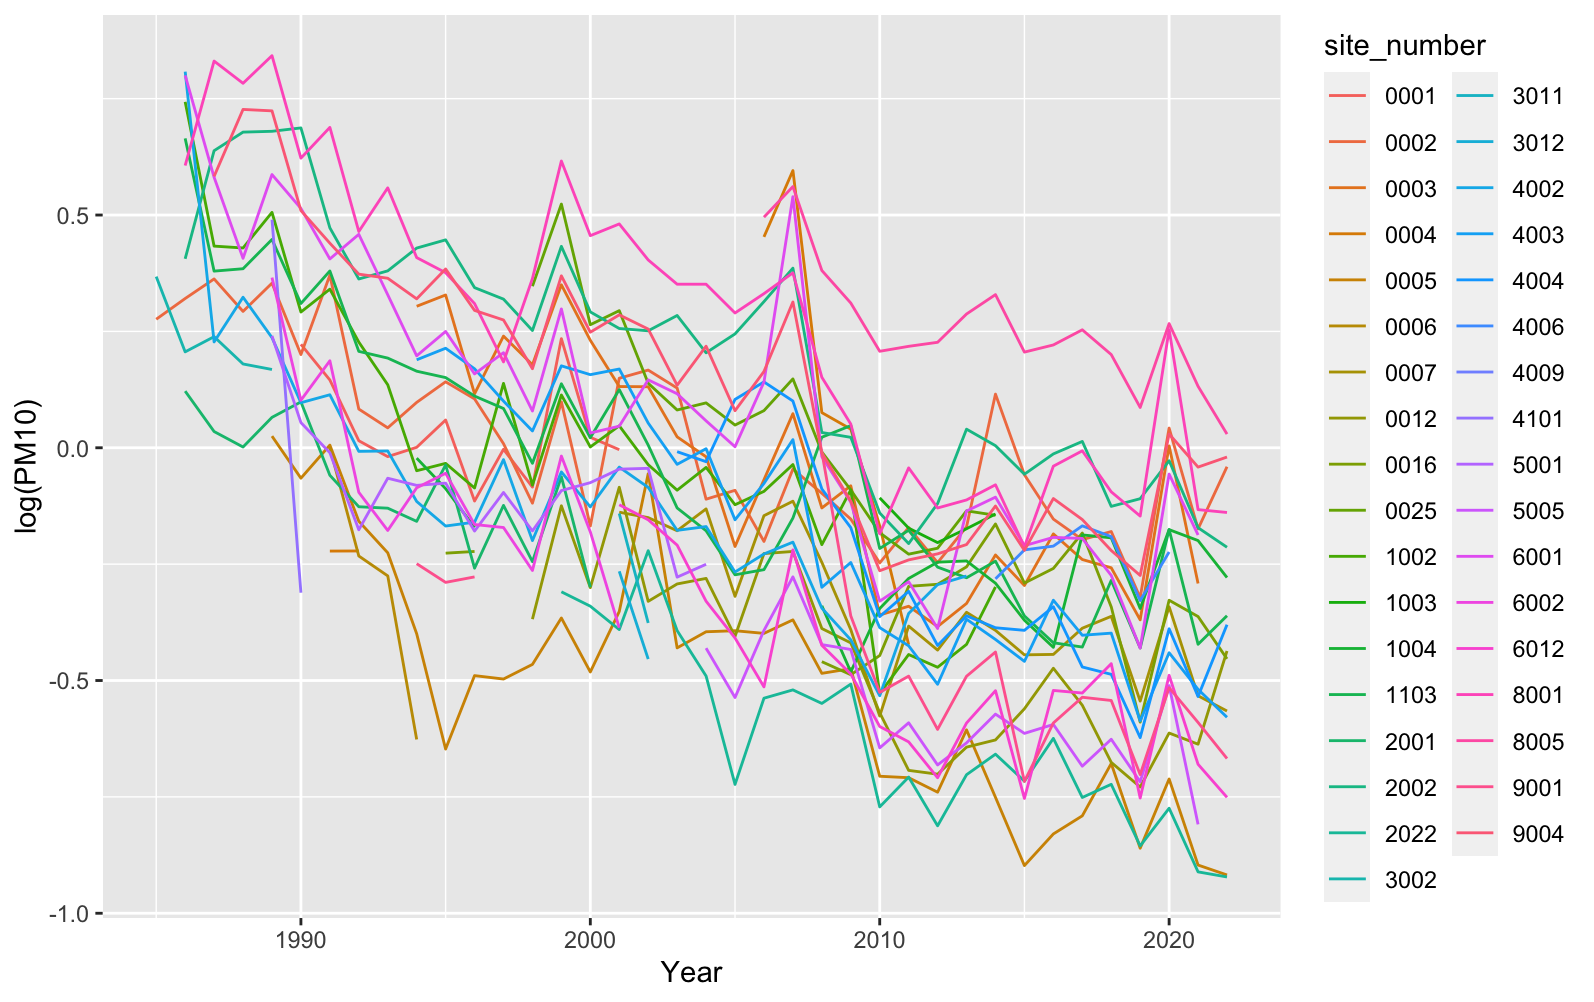
\includegraphics[width = 0.8\textwidth]{socab_plots/logPM10_traces.png}
	\caption{The sites in the SOCAB region.}
	\label{fig:logpm10_traces}
\end{figure}

\begin{figure}[ht]
	\centering
	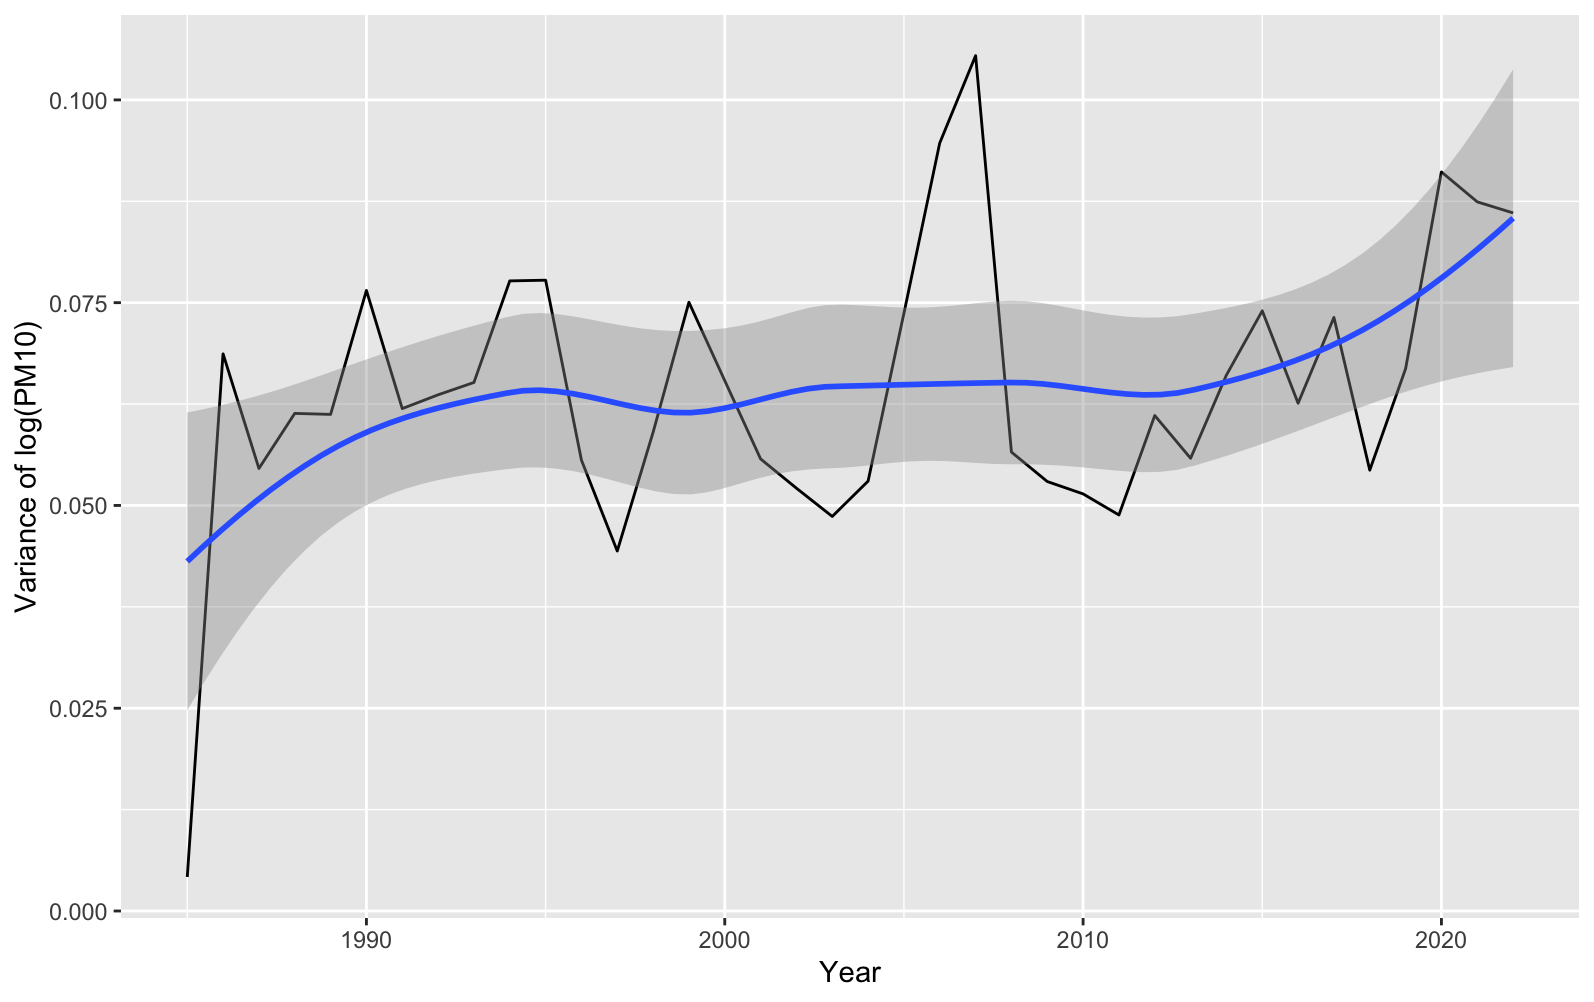
\includegraphics[width = 0.8\textwidth]{socab_plots/logPM10_var.png}
	\caption{The sites in the SOCAB region.}
	\label{fig:logpm10_var}
\end{figure}

\subsection{Map projection and Mesh Grid}
The site locations in the data set are recorded as latitude and longitude under different coordinate
reference systems (CRS). In order to better represent the distance between sites, we project all 
site locations to the UTM (Easting/Northing) coordinates with the measurement unit being kilometer.

The border map of SOCAB region is also projected to the same CRS as the site locations, and we keep
the sites only in the SOCAB region. 

\begin{figure}[ht]
	\centering
	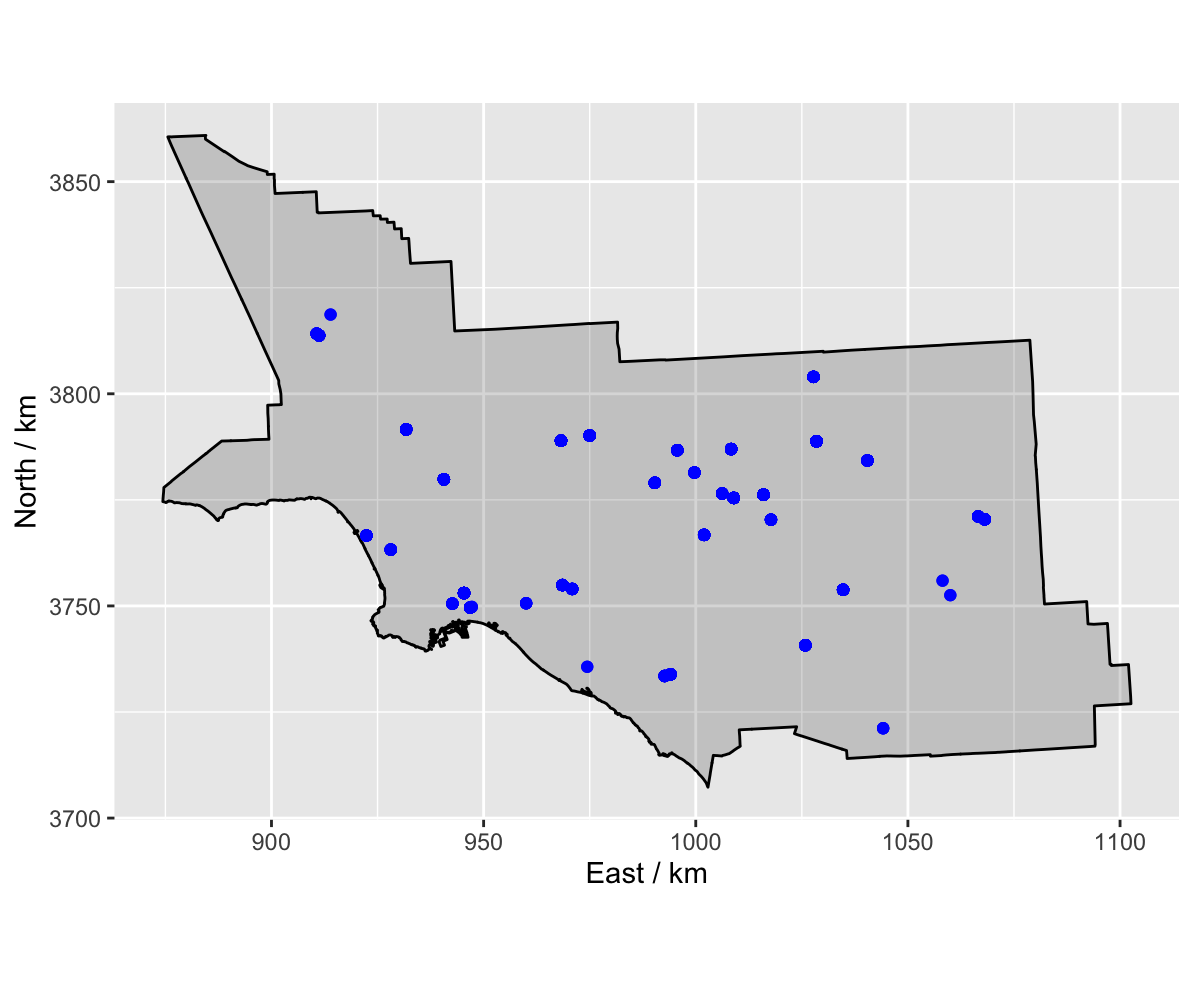
\includegraphics[width = 0.8\textwidth]{socab_plots/SOCAB_sites.png}
	\caption{The sites in the SOCAB region.}
	\label{fig:socab_sites}
\end{figure}

\begin{figure}[ht]
	\centering
	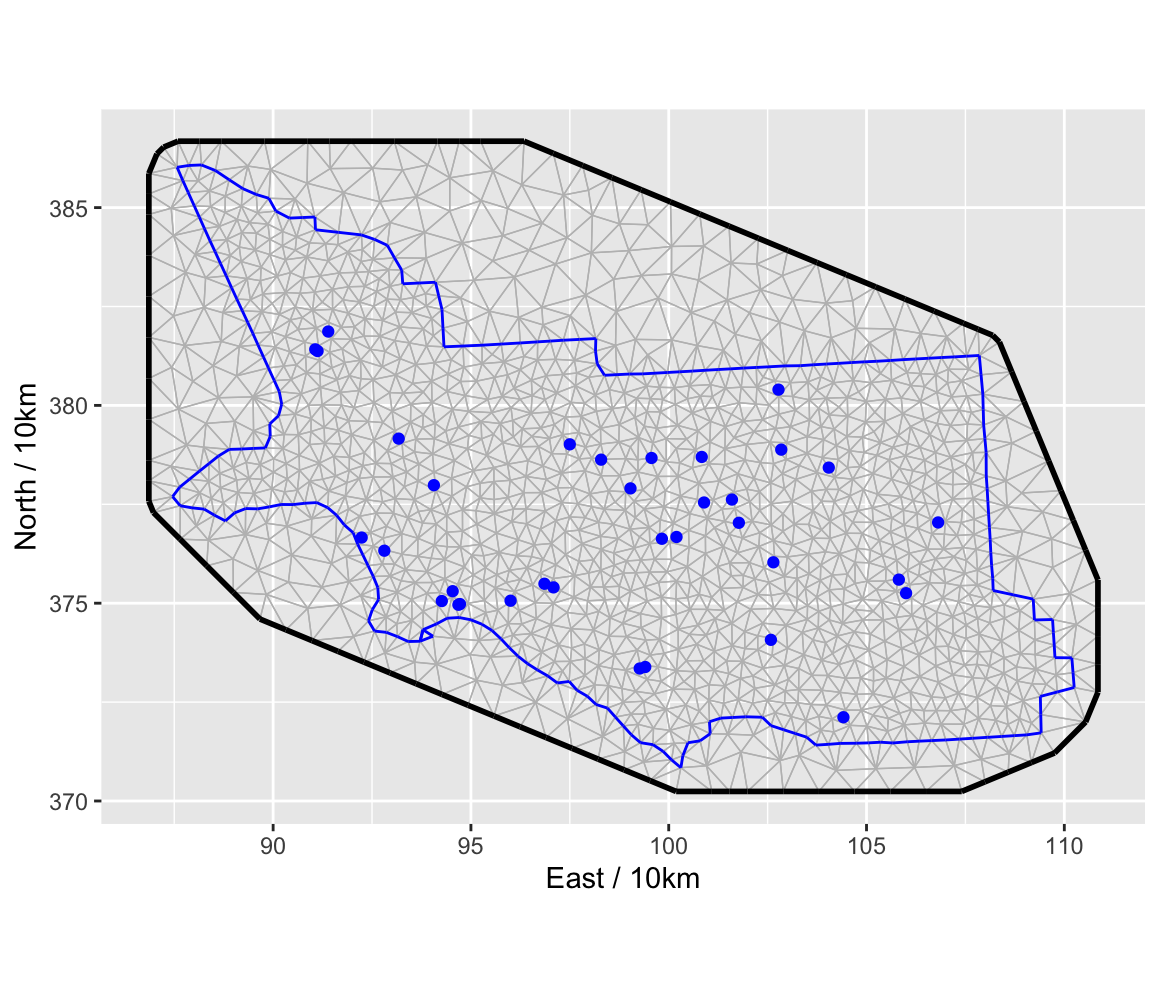
\includegraphics[width = 0.8\textwidth]{socab_plots/SOCAB_meshgrid.png}
	\caption{The meshgrid in the SOCAB region.}
	\label{fig:socab_meshgrid}
\end{figure}

To increase the numerical stability in model fitting, we rescale the Eastings and Northings 
coordinates of sites and the SOCAB border by 10, and each unit distance represent 10 km.

We create the mesh grid using the function $mesh_2d_inla$. 

The same mesh is used in both implementations. 


\section{Model Fitting}
In spatial statistics it is common to formulate mixed-effects regression models in which the linear predictor is made of a trend plus a spatial variation
The trend usually is composed of fixed effects or some smooth terms on covariates, while the spatial variation is usually modeled using correlated random ffects.
Spatial random effects often model (residual) small scale variation and this is the reason why these models can be regarded as models with correlated errors.

Lindgren et al. (2011) describe an approximation to continuous spatial models with a Matérn
covariance that is based on the solution to a stochastic partial differential equation (SPDE). 
A Gaussian spatial process with Matérn covariance is a solution to SPDE
This approximation is computed using a sparse representation that can be effectively implemented using the integrated nested Laplace approximation (INLA, Rue et al., 2009)

INLA focuses on models that can be expressed as latent Gaussian Markov random fields (GMRF)

INLA can handle models with more than one likelihood. By using a model with more than one likelihood it is possible to build a joint model with dfferent types of outputs and the hyperparameters in the likelihoods will be fitted separately.

We fit the same model on two populations using R-inlabru package. Inlabru is built upon the R-INLA 
package with simplified syntax. The R-INLA package apply the SPDE approach to add the
This enables the rapid computation of approximate Bayesian posterior distribution of the model 
parameters and random effects. The R-INLA packages approximates the Gaussian Markov random field by
solving an SPDE on a triangulation grid.
The goal of inlabru is to facilitate spatial modeling using integrated nested Laplace approximation via the R-INLA package.

\begin{lstlisting}[language = R]
	mesh1 <- inla.mesh.2d(loc = PM10.INLA.data.aea.SOCAB@coords, 
	boundary = SOCAB_union_sp,
	offset = c(1,40),
	max.edge = c(20, 40),
	min.angle = c(21, 21),max.n=c(48000, 16000), 
	max.n.strict=c(128000, 128000), 
	cutoff=5
	) 
\end{lstlisting} \label{code:inlaMesh}